\documentclass{sigchi}

\toappear{Submitted to CHI2014. Do not cite or distribute.}

\pagenumbering{arabic}

\usepackage{balance}  
\usepackage{graphics} 
\usepackage{times}    
\usepackage{url}      
\usepackage{gensymb}
\usepackage{afterpage}
\usepackage{mathpazo,amsmath}
\def\inch#1{#1''}
\def\ft#1{#1'\thinspace}

\makeatletter
\def\url@leostyle{%
  \@ifundefined{selectfont}{\def\UrlFont{\sf}}{\def\UrlFont{\small\bf\ttfamily}}}
\makeatother
\urlstyle{leo}

\def\pprw{8.5in}
\def\pprh{11in}
\special{papersize=\pprw,\pprh}
\setlength{\paperwidth}{\pprw}
\setlength{\paperheight}{\pprh}
\setlength{\pdfpagewidth}{\pprw}
\setlength{\pdfpageheight}{\pprh}

\usepackage[pdftex]{hyperref}
\hypersetup{
pdftitle={SIGCHI Conference Proceedings Format},
pdfauthor={LaTeX},
pdfkeywords={SIGCHI, proceedings, archival format},
bookmarksnumbered,
pdfstartview={FitH},
colorlinks,
citecolor=black,
filecolor=black,
linkcolor=black,
urlcolor=black,
breaklinks=true,
}

\newcommand\tabhead[1]{\small\textbf{#1}}

\newcommand {\bjoern}[1]{{\color{red}\bf{BH: #1}\normalfont}}
\newcommand {\ben}[1]{{\color{blue}\bf{BZ: #1}\normalfont}}
\newcommand {\sean}[1]{{\color{blue}\bf{SC: #1}\normalfont}}
\newcommand {\claire}[1]{{\color{blue}\bf{CT: #1}\normalfont}}
\newcommand {\studyquote}[1]{\em ``#1''\normalfont}

\begin{document}

\title{A Context Menu for the Real World: Controlling Physical Appliances Through Head-Worn Infrared Targeting}

\numberofauthors{1}
\author{
 \alignauthor Anonymous for submission
}

\maketitle

\begin{abstract}
 % abstract
We introduce a novel method for selecting and controlling smart appliances in physical spaces through a head-worn computing device with near-eye display and wireless communication. We augment a commercial wearable computing device, Google Glass, with a narrow-beam IR emitter for this purpose. This configuration yields a usable beam width of 2 to 4 feet (60 to 120cm) for targeting at room scale. We describe a disambiguation technique if infrared targeting hits multiple targets simultaneously. A target acquisition study with 14 participants shows that selection using head orientation with our device outperforms list selection on a wearable device. We also report qualitative data from using our device to control multiple appliances in a smart home scenario.

\end{abstract}

\keywords{
	smart devices; universal remote control; wearable computing; glass
}

\category{H.5.m.}{Information Interfaces and Presentation (e.g. HCI)}{Miscellaneous}

 % introduction
\section{Introduction}
Increasingly, devices and services in our built environment are networked and can be controlled remotely. The proliferation of smart, controllable devices such as intelligent lighting, AV equipment, HVAC systems, or kitchen appliances raises the question of how to best interact with them. 

Today, commercial solutions (such as Belkin WeMo) use handheld mobile devices as {\em universal remote controls} to control such appliances. In these solutions, users first browse a list of all available devices and then call up a device-specific user interface. This method faces two challenges: {\em naming} and {\em scoping}. Assigning clear names is non-trivial. In shared spaces, the person trying to control the device might not be the one that named it - e.g., while an office building manager may know what ``Light 4 in area E'' corresponds to, an occupant may not. Second, without a method of scoping selection to automatically filter non-relevant devices, paging though long lists of names or navigating hierarchies becomes potentially more cumbersome than the physical action the ``convenient'' software solution was meant to replace.

To address these challenges, research has introduced techniques of augmenting mobile devices with accessories like laser pointers to enable direct aiming at target devices~\cite{beigl_point_1999,patel_2-way_2003}. While promising, some drawbacks of using handheld devices are that the device first has to be retrieved (e.g., from a pocket) and aimed; that two hands may be necessary for operation (one to hold the device, one to operate the touch screen); and that the user's visual attention is now split between looking down at a screen and out at the device to-be-controlled. 

\begin{figure}[t]
\centering
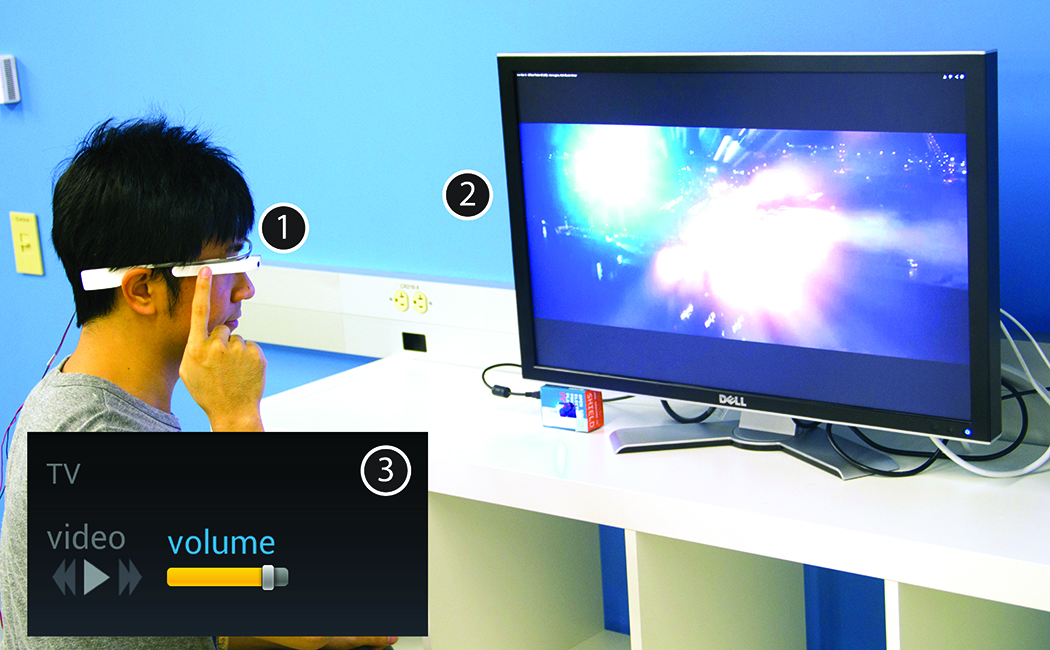
\includegraphics[width=1.0\columnwidth]{figures/teaser.jpg}
\caption{Using an augmented head-worn device (1), users can control smart home appliances (2) with head orientation targeting. A near-eye display then shows an appliance control UI (3), which users navigate through multitouch gestures.}
\label{fig:teaser}
\end{figure}

In this paper, we introduce a novel method for selecting and controlling smart appliances in physical spaces through the use of a head-worn computing device with near-eye display and wireless communication. We augment Google Glass\footnote{\url{http://www.google.com/glass/start/}} with custom hardware for this purpose. Users first look in the direction of the appliance they wish to control to initiate interaction (e.g., at a lamp to control lighting, or at a speaker to change music playback volume).  If multiple appliances fall within communication range, a disambiguation technique that combines on-screen information as well as visual feedback on the target appliances lets users select their desired target. Once acquired, an appliance specific control UI shown on the head-mounted display enables adjustment of discrete and continuous parameters through a touchpad interface (Figure~\ref{fig:teaser}).

Our hardware relies on infrared (IR) communication between Glass and target appliances to establish a connection; and on wireless 802.15.4 radio communication to exchange control messages.  Glass is augmented with a narrow-beam IR emitter and a 802.15.4 radio. Target appliances similarly have IR receivers and radios. This combination enables users to initiate interaction by orienting their head; but once initiated, users are free to look away from the target appliances while issuing control commands.

While prior work has tended to focus on proofs-of-concept, we also contribute empirical data on the system performance, usability, and user experience of head-orientation targeting and device control. We first report measurements of range and beam characteristics of our controller. We then conduct a study with $14$ participants that compares acquisition times for physical targets in a room for our technique and an alternative list selection interface. We find that target acquisition through head orientation is preferred by users and is faster than list selection, given the constraints of linear input using a head-worn touch controller. We also report qualitative results from participants who use our system for home automation tasks.


 % relatedwork
\section{Related Work}
Relevant prior work exists in the areas of remote control of physical appliances, evaluations of pointing in physical space and augmented reality applications. We discuss each in turn.

\subsection{Remote Control of Physical Appliances}
Standard infrared remote controls for televisions and AV equipment are only meant to control a single device. These controllers tend to use wide-angle infrared LEDs. Universal remote controls are available as dedicated devices (e.g, Crestron\footnote{\url{http://www.crestron.com}}) or applications for smart phones (e.g., Belkin WeMo\footnote{\url{http://www.belkin.com/us/wemo}}). They do not offer spatial selection of target devices, forcing users to browse through lists of pre-configured devices instead. Rukzio found that users strongly preferred either touching a mobile device to a target appliance or pointing at a distance to list browsing~\cite{rukzio_experimental_2006}.

Several approaches to spatial selection with handheld devices exist to control appliances~\cite{beigl_point_1999,patel_2-way_2003,wilson_xwand:_2003,schmidt_picontrol:_2012} or to exchange information with smart infrastructure sensor networks ~\cite{lifton_tricorder:_2007,mittal_ubicorder:_2011,costanza_sensortune:_2010}. Key design decisions are the method by which a target device is selected; and the method by which it is then later controlled or configured.

In several techniques, users select objects of interest with laser pointers. The laser dot provides immediate visual feedback to the user what is being selected (though it does not indicate whether the pointed-at object can indeed be controlled). Furthermore, laser pointer becomes obtrusive when there are other people in the space. Beigl's early AIDA handheld combines laser pointing with IR communication to exchange commands~\cite{beigl_point_1999}. Patel extends this technique by modulating the laser light to communicate the controllers' identity~\cite{patel_2-way_2003} to initiate radio communication. These proofs-of-concept do not include thorough evaluations. Kemp et al. use a laser pointer to indicate to robots which item to pick up in a room~\cite{kemp_point-and-click_2008}. 

The XWand~\cite{wilson_xwand:_2003} determines its absolute position and orientation and uses a virtual room model to select target devices. Position is determined through two ceiling-mounted cameras; orientation is determined using a built-in IMU. Users can employ physical gestures or utter speech commands to control selected devices. This technique requires room instrumentation and an up-to-date virtual model of device locations. The Tricorder~\cite{lifton_tricorder:_2007} uses IMU orientation coupled with room-localization based on received signal strength indicators (RSSI) to estimate what a user is pointing at.

Handheld projectors can both display a user interface in space and communicate control information optically, e.g., by encoding information temporally (using Gray codes in Picontrol~\cite{schmidt_picontrol:_2012} and RFIG~\cite{raskar_rfig_2004}) or spatially (using QR codes in the infrared spectrum in SideBySide~\cite{willis_sidebyside:_2011}). Printed tags like QR codes can also be affixed to devices and read by cameras. Common tagging systems are optimized to be read from a close distance, though it is possible to redesign codes that can be read further away (by encoding less information)~\cite{cross_low-cost_2012}. 

Our main area of differentiation is that we employ head orientation as the selection mechanism instead of pointing --- the user looks at the target device to initiate interaction. Selection techniques with very small selectors such as laser dots are less appropriate for head-mounted applications. We therefore select a source with a wider angle of illumination (an IR LED), but restrict its angle to be narrower than in general purpose IR applications.

\subsection{Evaluation of room-scale selection}
Pausch et al.'s early investigation of head-mounted displays compared head-tracking to handheld orientation control for a target acquisition task in a virtual reality room shown on a head-mounted display~\cite{pausch_user_1993}. They found a clear performance benefit for head-tracking.

On the other hand, Card et al. experimentally determined that the bandwidth of neck muscles is much lower than that of arm, wrist or finger muscle groups~\cite{card_morphological_1991}, which limits the performance of any head orientation-based interaction scheme. However, many other factors such as device characteristics and device acquisition time (e.g., pulling a phone out of one's pocket) contribute to overall performance and preference of different selection techniques.  Compared to a screen where every pixel is a potential target, the required accuracy for physical device selection in a room is much lower, and head orientation may provide sufficient accuracy. Our work only uses head orientation for the initial selection step; since we believe a user's attention is often drawn to the objects they intend to interact with. 

Myers et al compared different methods of interacting with displays at a distance~\cite{myers_interacting_2002} and quantified selection time and jitter or position error when using remote handheld pointing. Various techniques outperformed laser pointers. 

Our work is complementary as it provides concrete performance data on using head orientation to select targets in a physical environment.

\subsection{Augmented Reality Interfaces}
Augmented reality applications overlay digital information and graphics on the real world, e.g., through head-mounted displays~\cite{azuma_recent_2001} or other wearable devices. 
Our work is somewhat orthogonal to the research focus of this field as our device's graphics are shown in the visual periphery; they are not referenced to particular objects in the world, though our techniques could be extended to such configurations.


 % interaction
\section{Initiating Interaction through Attention}
This section describes the design goals of our system and their realization in particular interaction techniques.

\subsection{Design Goals}
Our work is motivated by the following design goals that leverage opportunities of head-worn computing, but also acknowledge potential challenges:

{\bf Leverage visual attention:} Take advantage of the fact that visual attention can express intention - initiate interaction based on where a user is already looking. 

{\bf Provide immediate feedback about selection targets in the environment:} While a near-eye display can push information to the user, users don't always want to control an object simply because they are looking at it (a problem known in gaze-based interaction as the Midas touch). A calmer~\cite{weiser_coming_1997} approach is to locate visual feedback about selection targets in the environment, to prevent distraction and interruption. Such feedback should be delivered instantaneously, while users look around a room.

{\bf Offer flexible orientation after initiating interaction:} After initiating interaction through head orientation, enable the user to reorient their head or body position during the remaining interaction to prevent neck strain.

{\bf Offer efficient ways to disambiguate orientation input:} It may not always be possible to identify a unique target appliance based on a user's attention and orientation. Offer ways to supplement orientation-based interaction with screen-based interaction to provide disambiguation information.

These design goals find their expression in the following interaction model.

\subsection{Interaction Flow}

\begin{figure}[t!]
\centering
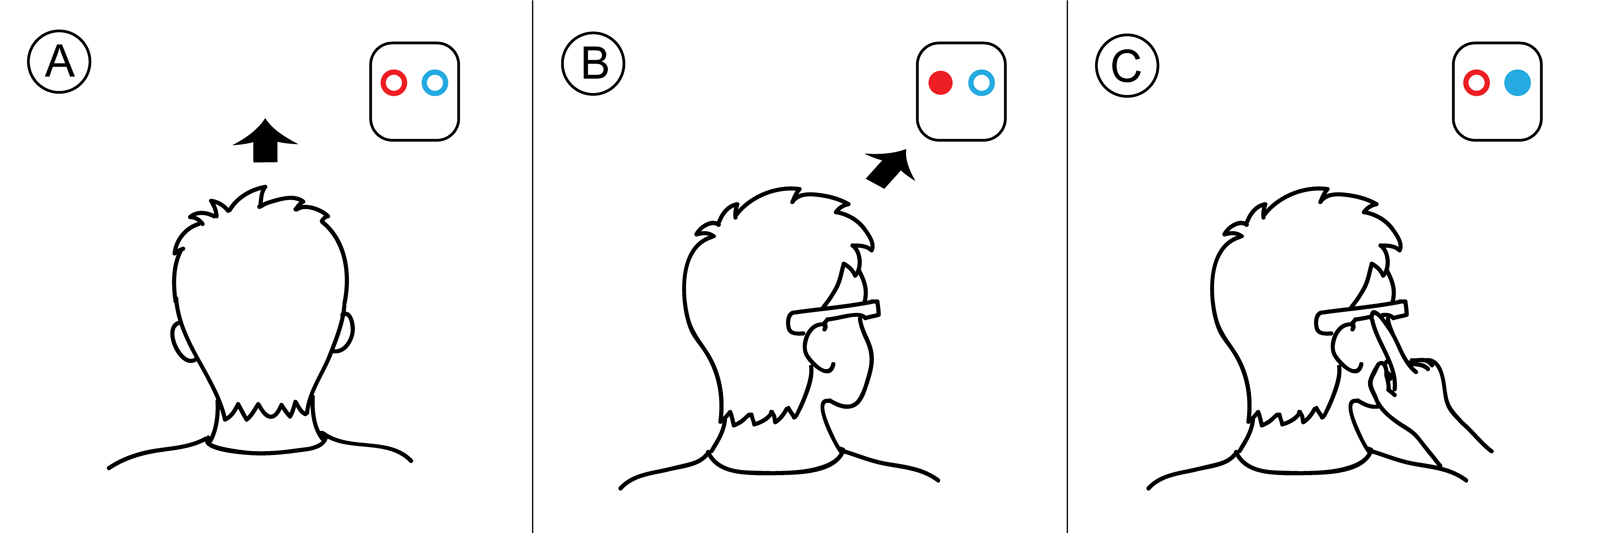
\includegraphics[width=\columnwidth]{figures/stepbystep_small.png}
\caption{Targeting interaction: when users turn towards a controllable appliance (A$\rightarrow$B), the appliance shows immediate visual feedback (red LED) (B). Users confirm that they wish to connect to this appliance with a tap (C) which triggers connection feedback (blue LED) on the appliance.}
\label{fig:interaction}
\end{figure}

\begin{figure}[t!]
\centering
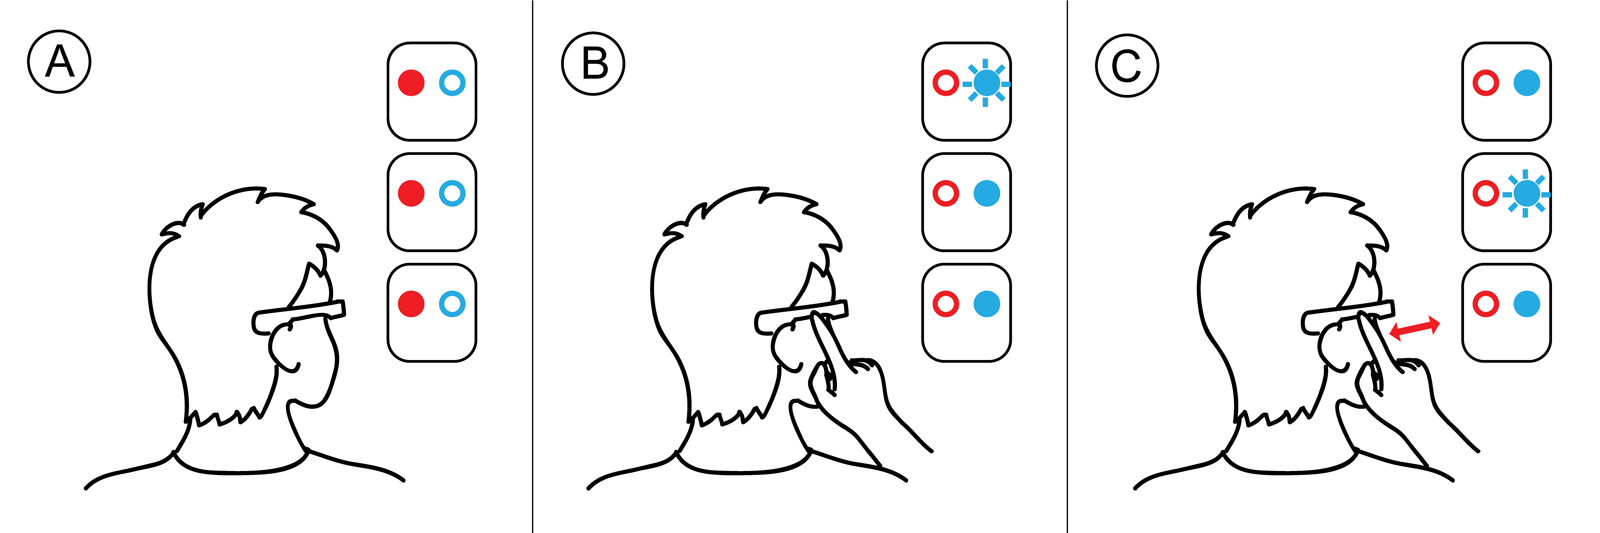
\includegraphics[width=\columnwidth]{figures/stepbystep_multi_small.png}
\caption{When multiple appliances are within range, they all have red LEDs illuminated for feedback (A). When users initiate connections, all target appliances toggle on blue LEDs while the currently selected one blinks (B). Swiping on the touchpad traverses among responding appliances (C).}
\label{fig:interaction_multi}
\end{figure}

{\bf Look:} Users select a target appliance by looking in its general direction.
Glass periodically sends a device id through its IR emitter analogous to Patel's approach~\cite{patel_2-way_2003}. Target appliances have IR receivers and offer immediate visual feedback by toggling a red LED whenever a valid id is received (Figure~\ref{fig:interaction}B). This enables {\em scanning} the environment with one's gaze to see which appliances can be controlled.

{\bf Initiate:} Users confirm their desire to connect to an appliance by tapping on the Glass touchpad. After they are connected, the target appliance toggles on a blue LED as visual feedback (Figure~\ref{fig:interaction}C). The next section on disambiguation deals with cases in which multiple appliances received valid IR signals. At this point, all further communication switches over to the 802.15.4 wireless network so that line of sight to the target is no longer needed.

{\bf Control:} Glass displays a user interface for parameters of the chosen appliance. Upon connection, the current status of the appliance is retreived by Glass and shown on the UI. The interface is controlled with the temple-mounted touchpad through the following gesture set: tapping toggles discrete parameters (such as power for a lamp as Figure~\ref{fig:ui_controls}(A)); single finger swipe changes between available parameters; double finger swipe adjusts continuous parameters (such as volume for a video player as Figure~\ref{fig:ui_controls}(B)). This scheme was chosen because the touchpad is only comfortably operable in the coronal plane (front to back) but not in the sagittal plane (up and down). 
Control commands are sent over XBee radios.

{\bf Disengagement:} Users stay connected to the last selected appliance up to a timeout period. During that period, users can disengage through down swipes.

\begin{figure}[t!]
\centering
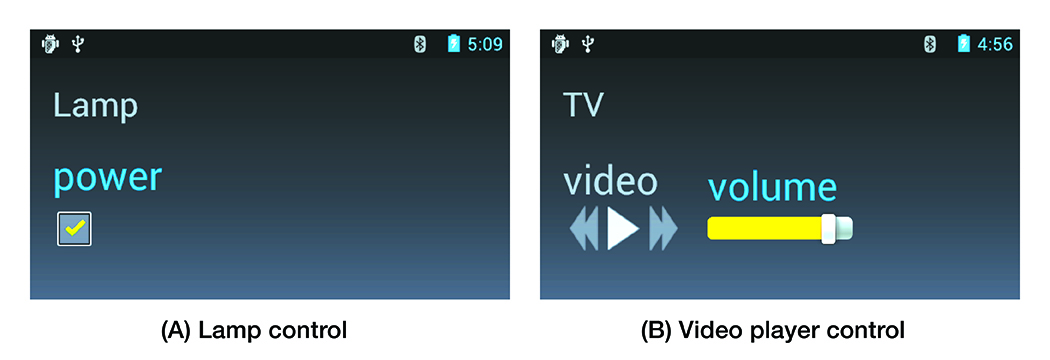
\includegraphics[width=\columnwidth]{figures/ui_controls_caption.jpg}
\caption{Two screenshots of UI controls for lamp and video player.}
\label{fig:ui_controls}
\end{figure}

\subsection{Disambiguation}
Head orientation only indicates a general area of visual interest. It does not necessarily match gaze orientation as extra-ocular muscles can move the eyes. The IR beam of our device also has a certain spread (see next section). In an environment dense with potential targets, multiple targets could be within range. Users can tell when multiple feedback LEDs in the environment illuminate (Figure~\ref{fig:interaction_multi}A). To disambiguate, users can either move to adjust their head position, or, alternatively, call up a disambiguation dialog on the Glass display. The dialog presents a list filtered to only those appliances that are within IR range, while appliances also use blue LED as visual cues: all responding appliances light up LEDs while the currently selected one blinks (Figure~\ref{fig:interaction_multi}B). Users navigate the list using the touchpad (Figure~\ref{fig:interaction_multi}C), and then continue their interaction as described above.

 % device

\section{Hardware Device}
\begin{figure}[t]
\centering
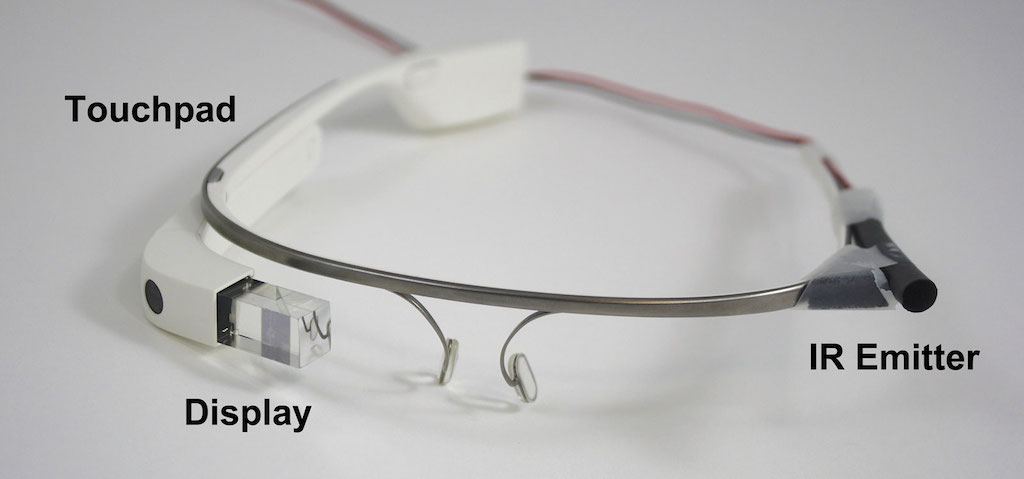
\includegraphics[width=1.0\columnwidth]{figures/glass-with-ir}
\caption{Our augmented Glass prototype has a frame-mounted infrared emitter.}
\label{fig:glass}
\end{figure}
\begin{figure}[t]
\centering
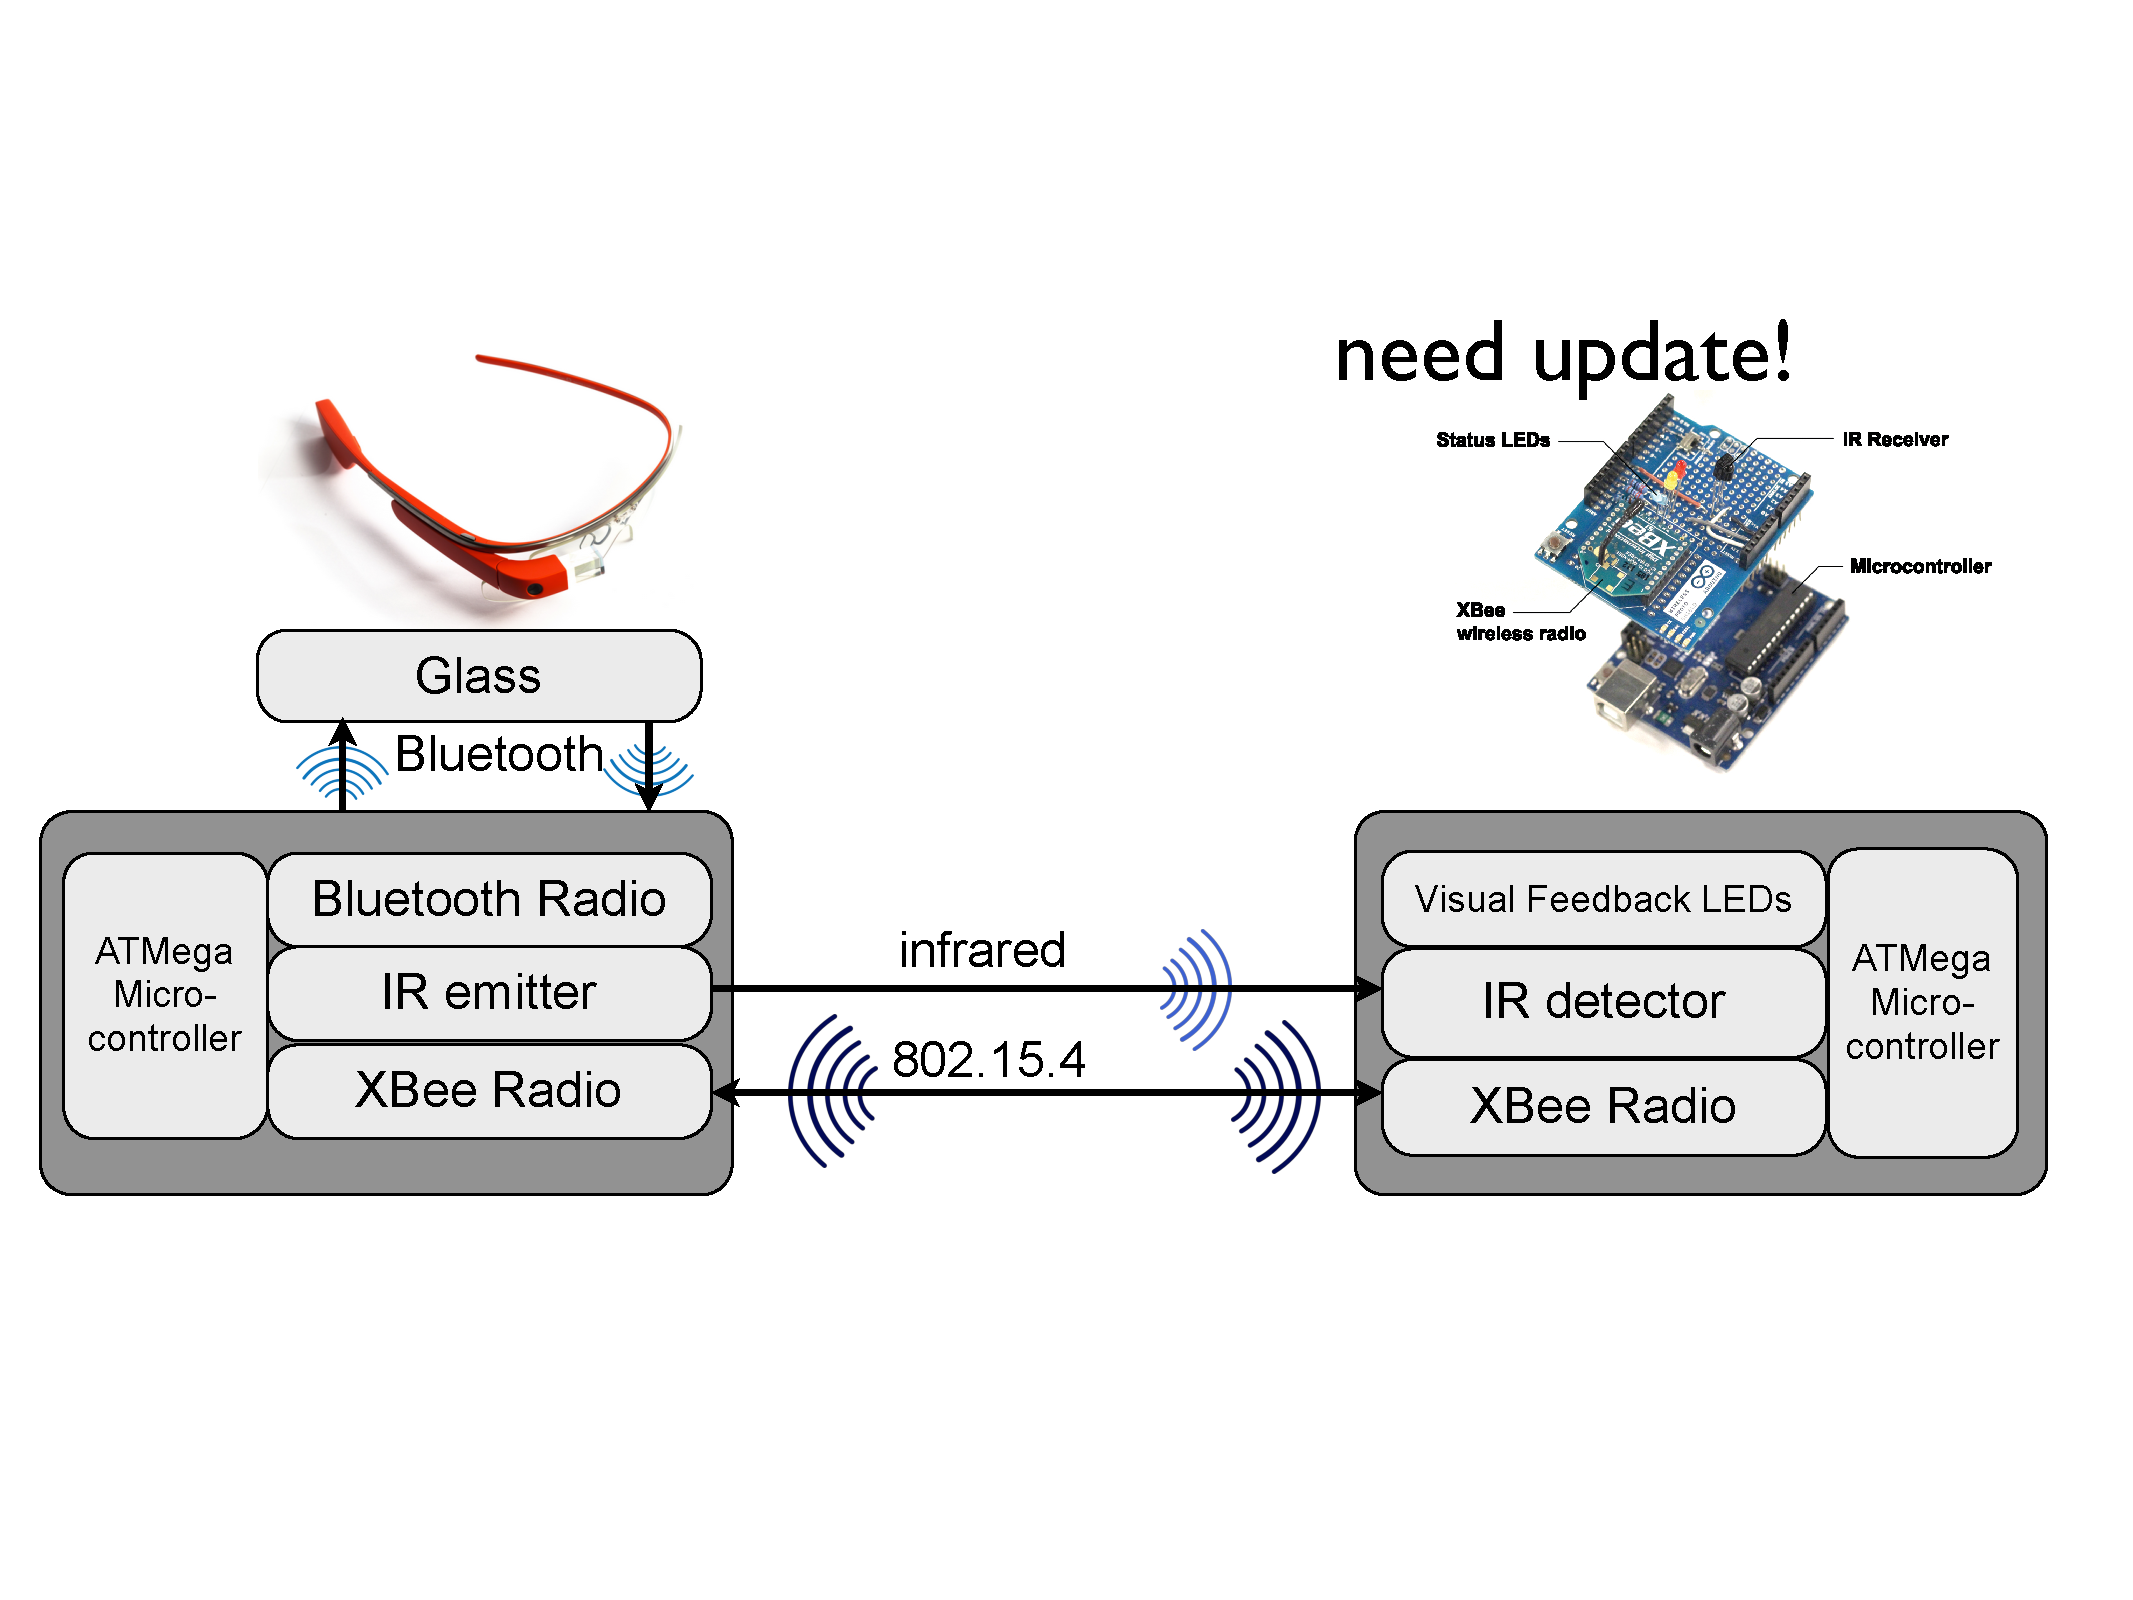
\includegraphics[width=1.0\columnwidth]{figures/architecture}
\caption{In our system architecture, selection is initiated through infrared but confirmed over 802.15.4. This permits wearers to move their head freely after connecting to an appliance. In the research prototype, users have to carry an additional microcontroller board that marshals messages between Glass' Bluetooth radio an IR/802.15.4, but our custom hardware could also be integrated into the wearable device.}
\label{fig:architecture}
\end{figure}

\subsection{Prototype Implementation}
Our prototype consists of a Google Glass Explorer Edition head-worn computing device, augmented with an infrared emitter that is mounted on the frame, pointing out in the direction of the wearer's view (Figure~\ref{fig:glass}). The IR emitter LED is mounted in an opaque hollow tube, that restricts the outgoing angle of illumination. 

In our prototype, Glass communicates over Bluetooth to an additional microcontroller board the user has to wear (Atmel ATMega256). This board marshals XBee to Bluetooth messages in both directions and also controls the IR LED mounted on the Glass frame (Figure~\ref{fig:architecture}). This architecture was mostly chosen for reasons of expediency. We selected XBee 802.15.4 radios to avoid Bluetooth  wake up latencies but we do not claim optimality for our design decisions. Future head-mounted devices could clearly integrate IR emitters; the choice of local wireless technology could also change. In particular, one could substitute WiFi modules or design an all-Bluetooth network.

\subsection{Device Characterization}
We determined the usable range and accuracy empirically with one IR emitter and two IR receivers. The IR emitter constantly sent out an id signal. The receivers that correctly received the signal turn their LED on for 300 ms.

We placed all three devices at the same height with clear line of sight. The IR emitter is first places 2 feet away from the receivers. The receivers were moved sideways apart from each other until they could no longer receive stable signals. We then recorded the distance of the two receivers for the calculation of coverage angles. The steps are repeated for IR emitters in different distances (as shown in Table~\ref{table:measurements}). We then repeated measurements with the emitter  placed at various depths in the tube (see Figure~\ref{fig:coverage}). 

In summary, our measurements suggest that IR communication can be targeted to an area about 2--4' in diameter, up to 16' in front of the user. These values are a reasonable match for selecting appliances in a room-size environment. A wider beam would lead to an increased chance of multiple appliances receiving IR signals simultaneously. A narrower beam will make targeting more challenging, given the precision constraints of human head movement.

\afterpage{
\begin{figure}[t!]
\centering
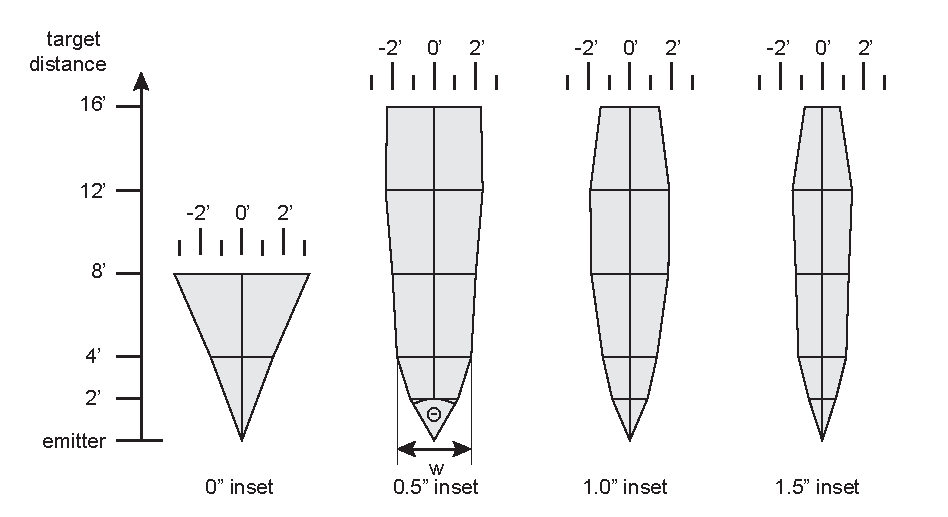
\includegraphics[width=1.0\columnwidth]{figures/glass-ir-coverage}
\caption{Different IR configurations suggest usable beam widths of 2 to 4 feet and distances up to 16 feet }
\label{fig:coverage}
\end{figure}

\begin{table}[h!]
    \begin{tabular}{l|lllll}
    distance/ depth & \ft2       & \ft4       & \ft8   & \ft{12}  & \ft{16}  \\ \hline
    \inch{0}                     & $74\degree$ & $78\degree$ & N/A  & N/A  & N/A  \\
  \inch{0.5}                   & $60\degree$ & $48\degree$     & $28\degree$ & $22\degree$ & $16\degree$ \\
    \inch{1.0}                     & $46\degree$     & $36\degree$     & $26\degree$ & $18\degree$ & $10\degree$ \\
    \inch{1.5}                   & $36\degree$     & $32\degree$     & $18\degree$ & $14\degree$ & $6\degree$  \\
    \end{tabular}
    \caption{Measured IR coverage angles $\Theta$ at different target distances and different depths of IR emitter inside shielding tube.}
    \label{table:measurements}
\end{table}
} 

 % targeting
\section{Physical Target Acquisition Study}
To understand the accuracy and performance of head-orientation-based  selection through our device, we carried out a comparative target acquisition study, where participants had to connect to wireless nodes distributed in a room with our technique, and with an alternate list selection approach.

\begin{figure}[t]
\centering
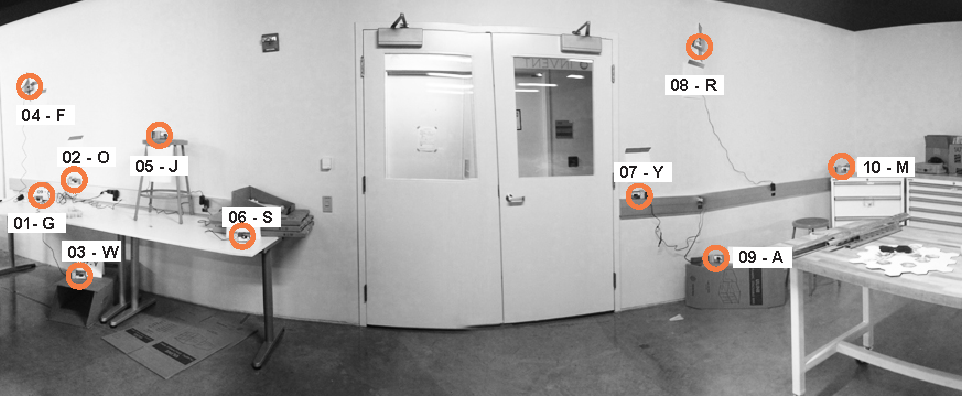
\includegraphics[width=1.0\columnwidth]{figures/targeting-study-layout.pdf}
\caption{In the targeting study, participants had to find and select one of 10 targets in a lab environment. Targets were called out by number; for the list mode condition, participants need to match numbers to letters.}
\label{fig:targeting-study-layout}
\end{figure}

\subsection{Apparatus}
In an indoor environment, 10 wireless nodes are spread across a room at various heights and distances (Figure~\ref{fig:targeting-study-layout}). The nodes are stand-ins for potential smart appliances and have all relevant functionality for targeting and wireless communication, but do not control any actual appliances. Each node is an embedded wireless system with a microcontroller, IR receiver, a wireless XBee radio, and three status LEDs (Figure~\ref{fig:target}). An yellow LED indicates that the device is the target that should be selected in the current trial; a red LED lights up whenever the device receives an IR signal from Glass; a blue LED shows when participants have successfully connected to a device, and is also used for disambiguation when multiple targets are within IR range. Next to each target, a paper sheet shows a number and letter combination, which is used for uniquely identifying the device. The numbers are the primary identifiers, ordered from left to right in the room. This ordering makes it easy to locate them, which simulates looking towards an appliance with a well-known location in a room, and minimizes visual search time.

\begin{figure}[b]
\centering
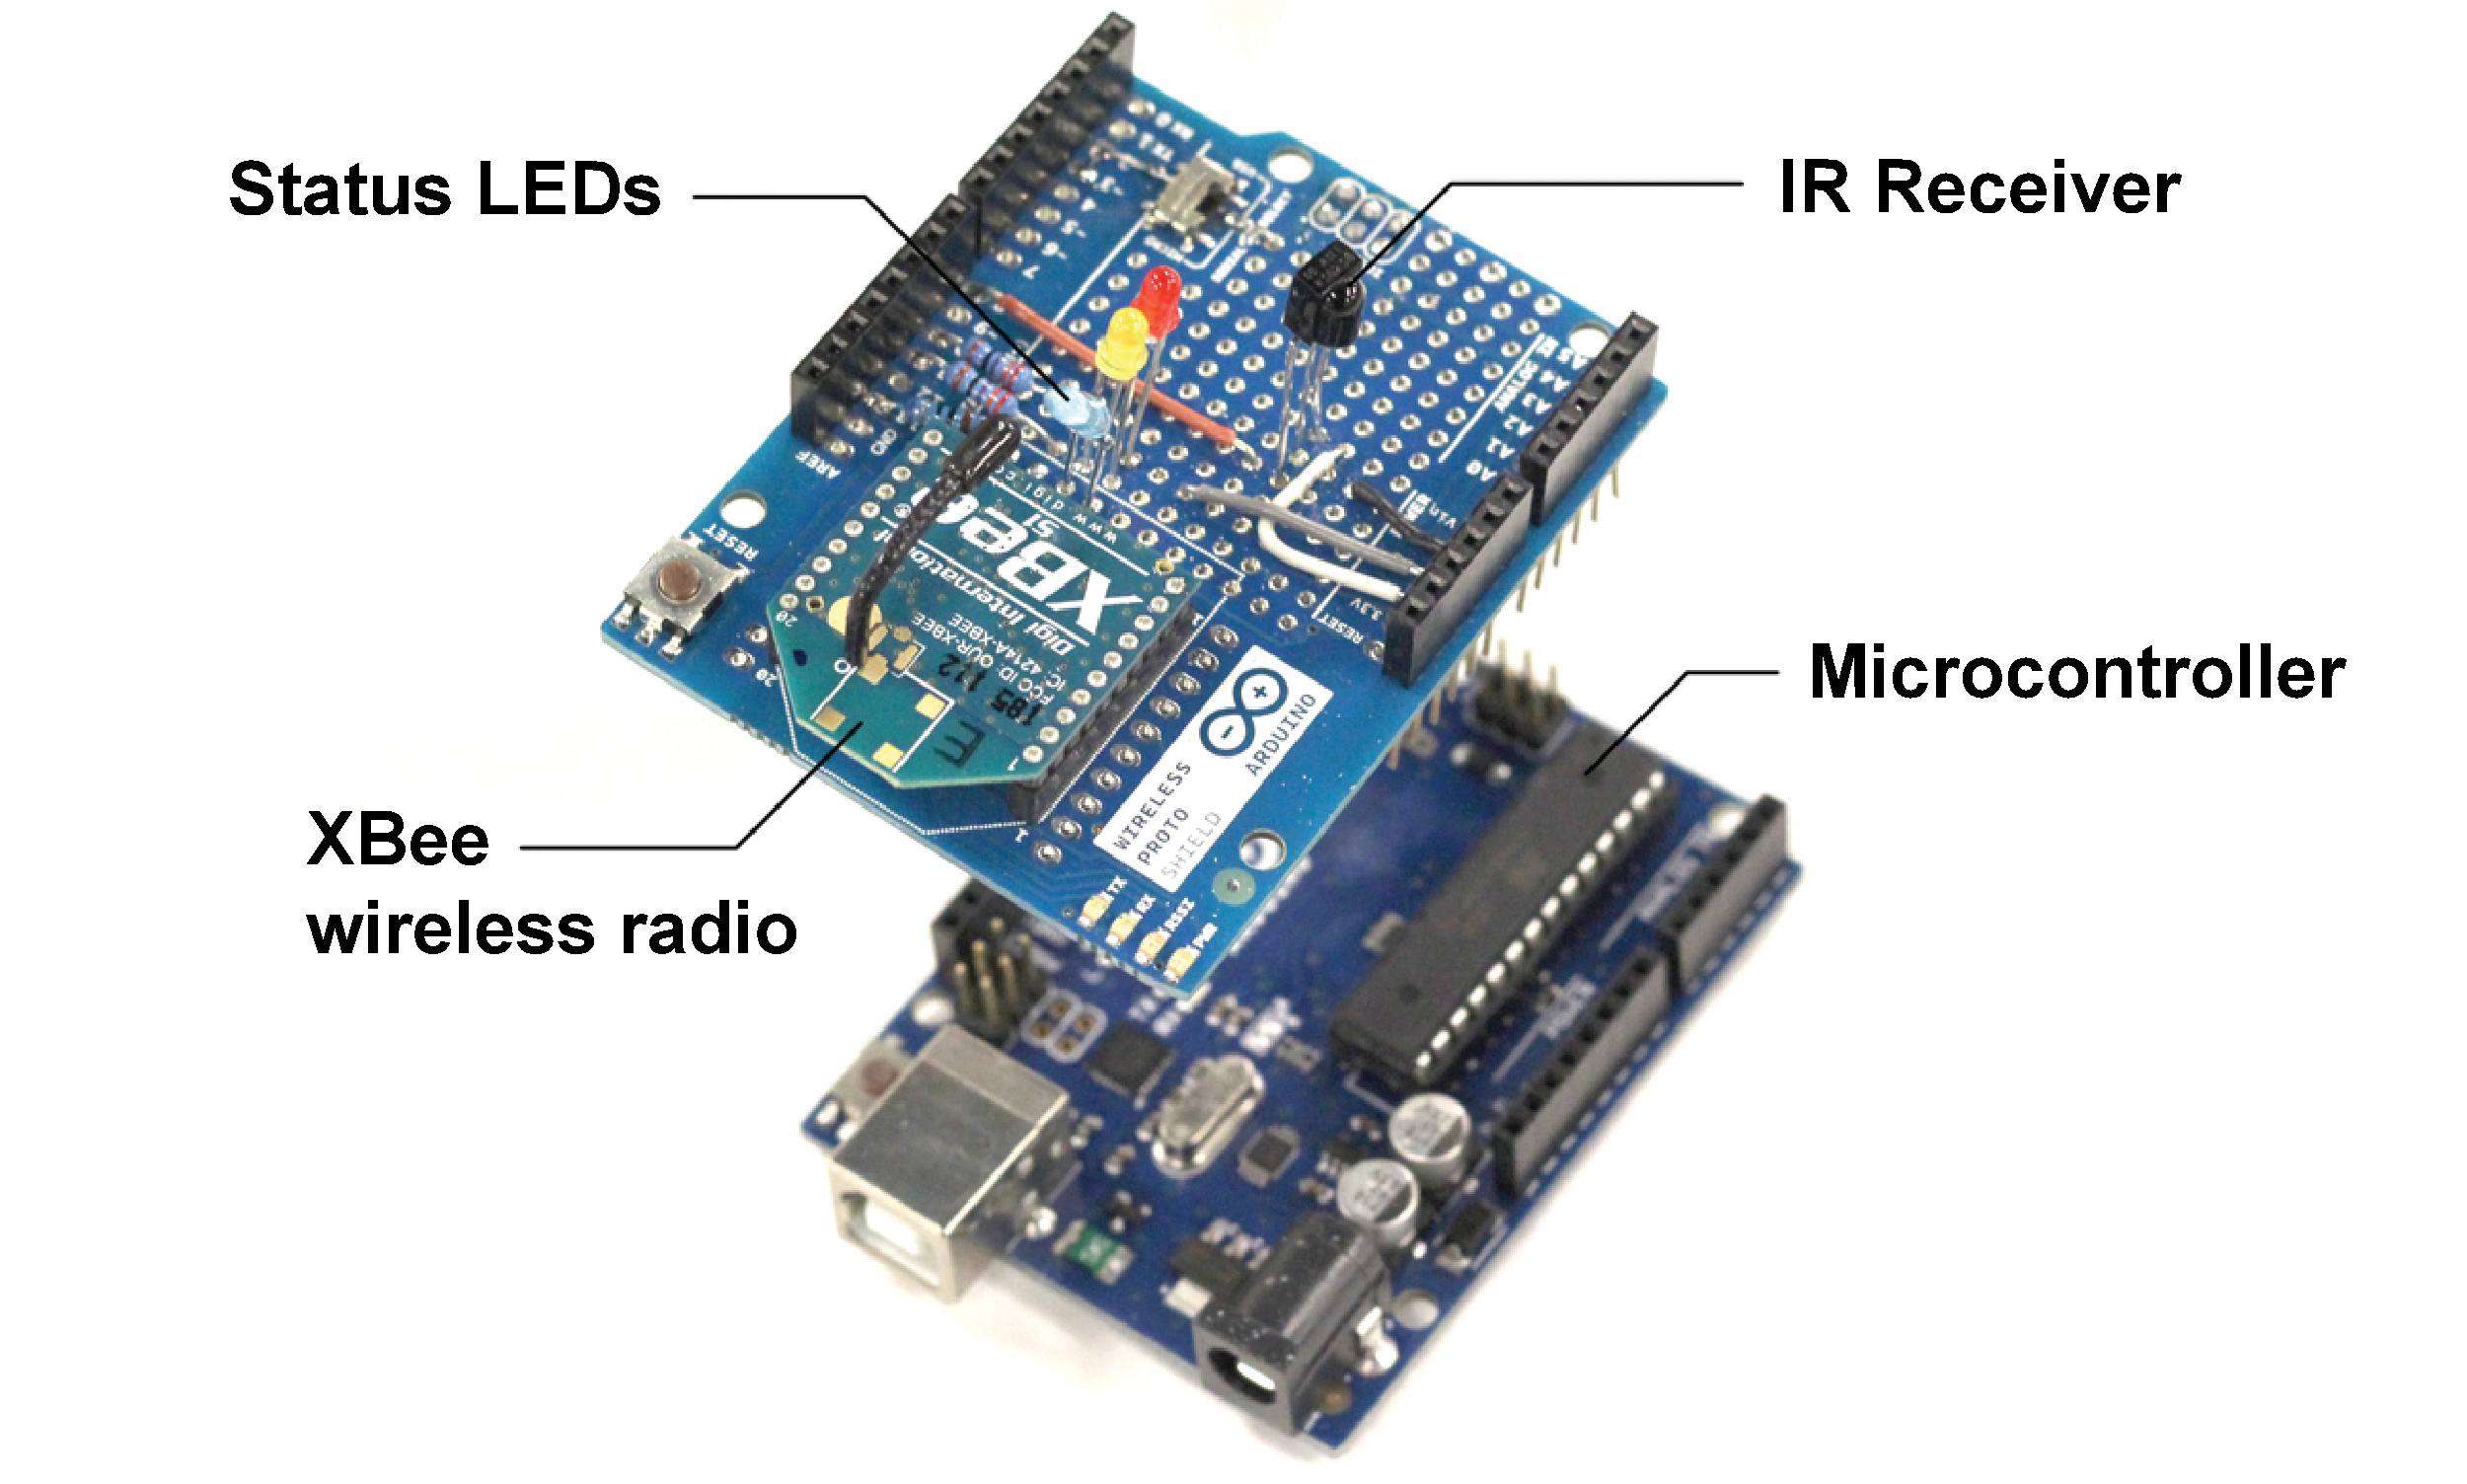
\includegraphics[width=0.8\columnwidth]{figures/study-node.pdf}
\caption{An example node from the targeting study --- we constructed 10 such nodes - each mounted in a box.}
\label{fig:target}
\end{figure}

\subsection{Methodology}
In our within-subjects design, participants performed 15 target acquisition tasks each with two interaction styles. In the {\em infrared} mode condition, participants used our IR targeting approach; in the {\em list} mode condition, participants had to look up a device's letter code on the printed paper next to the device and then select that letter code from a list displayed on their Glass device. The list was navigated with swipe motions on the Glass touchpad. For each task, participants started at a fixed position in the room. The experimenter called out a number and simultaneously started a timer. Participants then had to find the corresponding device (by looking for its printed code). In the {\em infrared} mode, participants then selected and acquired the target by aiming the IR beam at the target, and confirmed their selection with a touch pad tap. If more than one target was within range, participants had to either use the disambiguation dialog or reposition themselves. In the {\em list} mode, participants had to read the letter next to the number and then select that letter by browsing a linear list shown in their Glass display. While the list was alphabetized, letter arrangement in the room was not. This design required participants to find the target in the room before starting a list navigation to keep visual search times similar in each condition.

Afterwards, participants completed a survey that elicited answers to Likert-scale questions as well as open-ended answers about their experience.

\subsection{Participants}
We recruited 14 participants from our institution. 13 had never used Glass before. 4 wore prescription glasses, which may have affected their task performance as wearing glasses beneath Glass makes it more cumbersome to secure the position of Glass and to adjust the screen to the optimal angle. Half of them performed {\em infrared} mode first and the other half did {\em list} mode first.

\subsection{Measures}
The main measures were {\bf target acquisition time}: the time required to identify, select, and connect to a wireless target device; and {\bf user preference}: which interface users preferred for the task after completing the study.

\subsection{Results}
\subsubsection{Performance data}
The time to complete each task can be broken down into the following pieces:

$t_{infrared}=t_{locate}[+t_{reorient}][+t_{disambiguate}]+t_{tap}$

$t_{list}=t_{locate}+t_{listnav}+t_{tap}$

In both conditions, participants first have to locate the target announced by the experimenter through visual search ($t_{locate}$). In the {\em infrared} mode, participants may then directly confirm their selection if only a single target was selected ($t_{tap}$). However, if they don't immediately receive feedback that their target was selected, or if multiple targets were selected, users either have change their position or head orientation ($t_{reorient}$) or they have to step through the on-screen disambiguation dialog ($t_{disambiguate}$). In the {\em list} mode, participants must scroll through the list to find the desired target identifier ($t_{listnav}$).
Thus, {\em infrared} will show a performance benefit if $(t_{reorient}+t_{disambiguate})<t_{listnav}$. This depends on the number of total devices in the environment (increasing $t_{listnav}$), and their density (which will increase $t_{disambiguate}$). 

\begin{figure}[t]
\centering
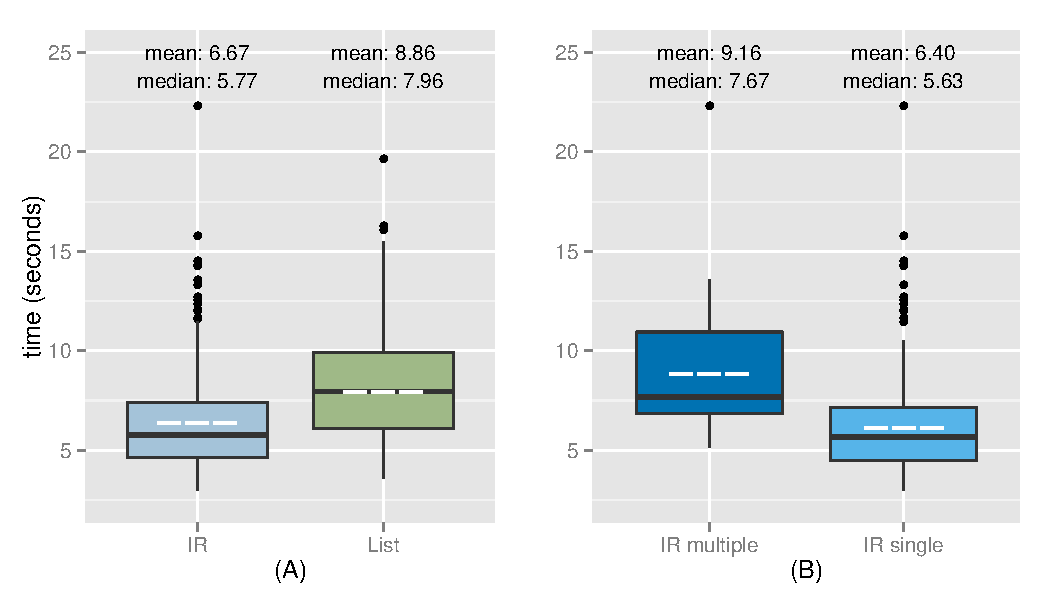
\includegraphics[width=1.0\columnwidth]{figures/R_time_by_Category.pdf}
\caption{Boxplot of task completion times for the comparison between {\em infrared} mode and {\em list} mode (A), and between IR multiple responses cases and IR single response cases (B). The centers of boxes are median values, while white dashed lines are mean values.}
\label{fig:selection-times}
\end{figure}

We first show results for 10 targets and then discuss extrapolations of these results. Average target acquisition time $t_{infrared}$ was 6.67 seconds, while $t_{list}$ was 8.86 seconds (Figure~\ref{fig:selection-times}A). This difference is significant (Student's t-test, $t(279)=-3.81, p=0.00017$). 

To further understand the performance gain in {\em infrared} mode, especially the factor $t_{disambiguate}$, we compare selection times when multiple devices are targeted (and disambiguation is required) to single-device selection times (Figure~\ref{fig:selection-times}B). When there is a single device, $t_{disambiguate}$ is 0 and it takes 6.40 seconds (on average) to complete the connection. When multiple devices are in range, the time increases to 9.16 seconds, indicating 2.76 seconds required to disambiguate. Though it takes significantly longer ($t(19)=-2.7827, p=0.012$ using t-test) in the {\em multiple} case, these cases made up only 10\% of total infrared trials.

\begin{figure}[t]
\centering
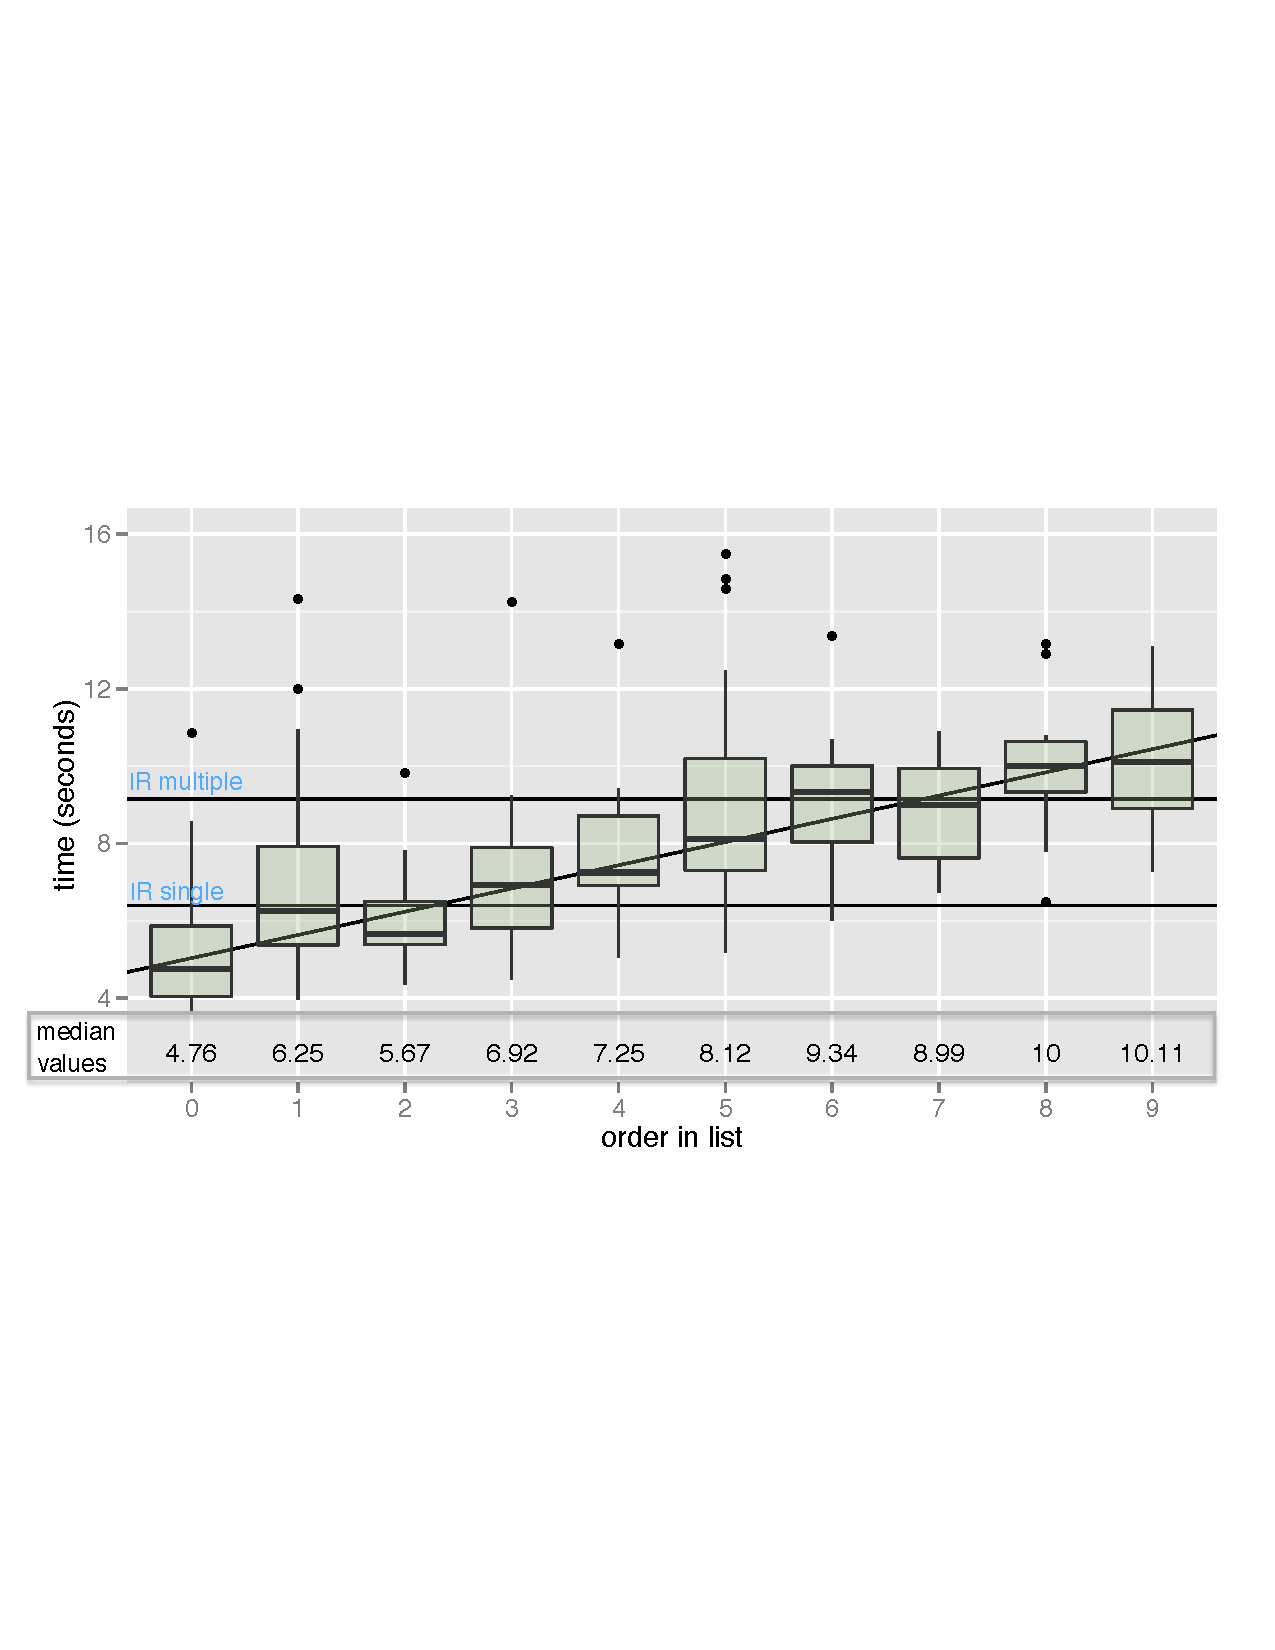
\includegraphics[width=1.0\columnwidth]{figures/R_List_by_Target.pdf}
\caption{Times taken to select a device vs.~its order in the list. The dotted line is a linear fit between the mean times and device orders. Two horizontal lines of mean target acquisition times in {\em infrared} mode are also annotated for comparison.}
\label{fig:time-vs-list-order}
\end{figure}

For each device, $t_{listnav}$ depends on their relative position in the list. Figure~\ref{fig:time-vs-list-order} shows the time it takes to select a device (means and standard deviations) as a function of its list position - the trend line (dotted) enables extrapolation to estimate at what number of devices the {\em infrared} mode interaction techniques will outperform {\em list} mode\footnote{The higher mean value at $order=1$ is caused by one outlier when the participant tried multiple times in {\em list} mode to connect to the right target.}. From the figure, we can see that once the target's order has increased to be larger than 6, the average $t_{listnav}$ for that target would be larger than $t_{reorient} + t_{disambiguate}$. We expect that, when the number of targets keeps increasing, there would be larger time reduction in {\em infrared} mode.

Participants' selection errors do occur in both conditions. However, error rates were low (1.1\% in {\em infrared} mode, and 2.9\% in {\em list} mode, respectively). This precludes us from running a more detailed analysis. 

\begin{figure}[t]
\centering
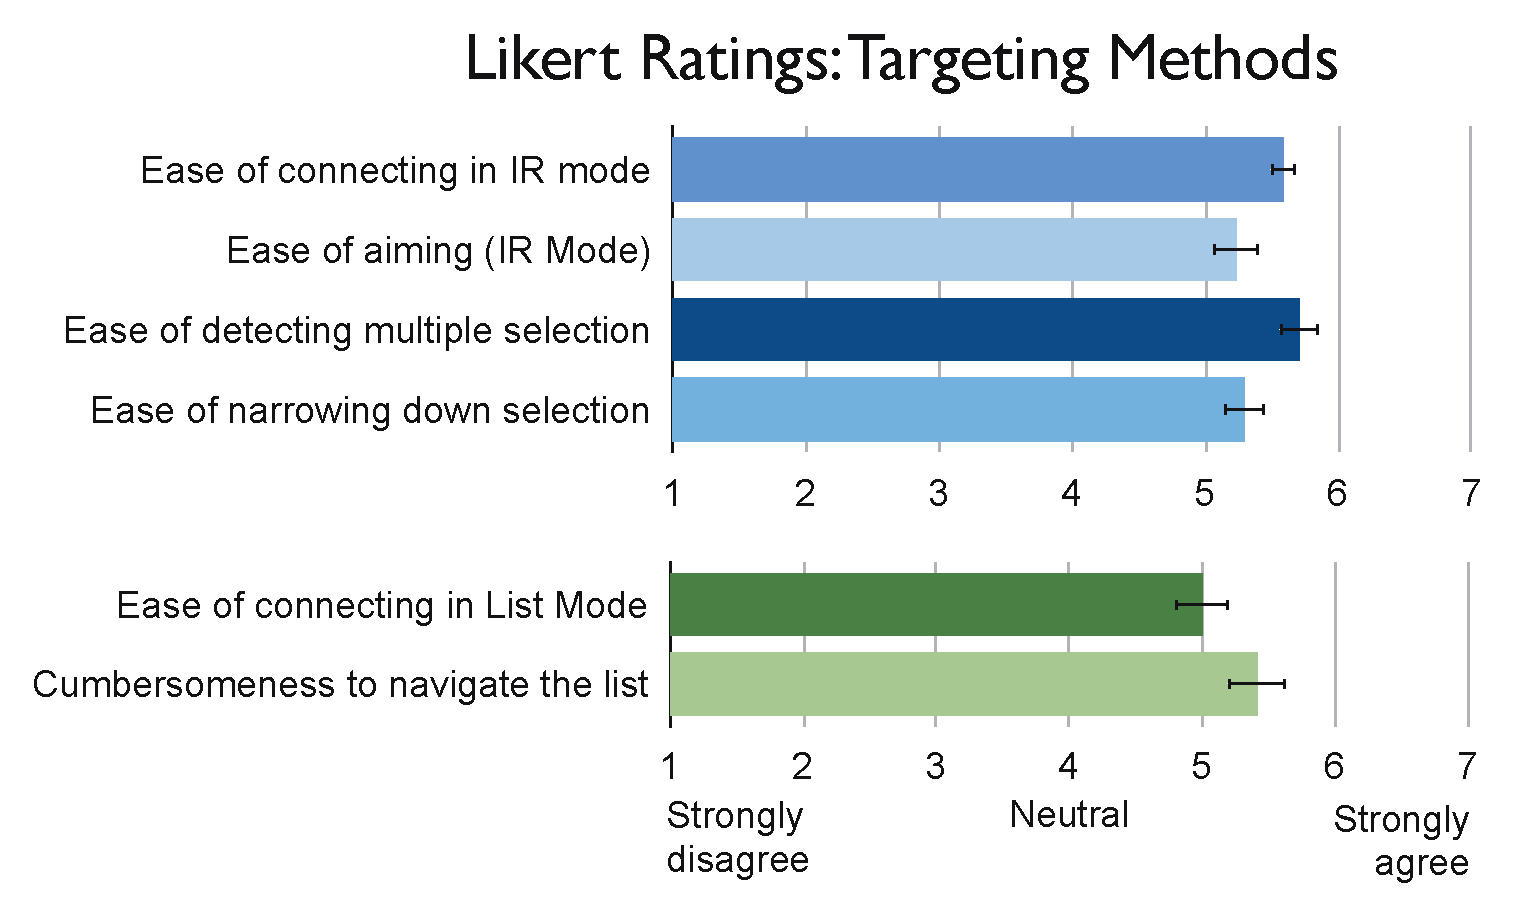
\includegraphics[width=1.0\columnwidth]{figures/target-likert.pdf}
\caption{Likert scale ratings for ease of use of aspects of the targeting task. Error bars show standard error. }
\label{fig:target-likert}
\end{figure}

\subsubsection{Preference}

Eleven of 14 users preferred infrared mode over list mode (three preferred list, one was undecided). While both interfaces were judged similarly on overall ease of connecting, list navigation was also perceived to be cumbersome (see Figure~\ref{fig:target-likert}). As self-report data can easily skew positive as participants try to please experimenters, we also asked participants to elucidate why they preferred one interface over the other.

List mode had certain advantages: It was judged to be more accurate and predictable as there was always exactly one device selected in the list (\studyquote{With the list you never have to worry about accidentally picking up two targets}). Also, it did not require a clear line of sight to the target device so participants did not have to move from their starting position (\studyquote{The shortcoming of the IR mode was that you had to be a certain distance away in order for it to detect the appliance}). 

On the other hand, list mode was judged to be more \studyquote{annoying} and tedious. The temple-based touchpad for selection was difficult to use for a participant with long hair: \studyquote{List mode was physically difficult for me to navigate, since my long hair wasn't tied back and it kept interfering with my swiping.} Another participant also commented on the ergonomic challenge of touchpad use on Glass: \studyquote{The strength of the IR mode was that I didn't have to use my fingers as much to control. If the items were spaced relatively far apart, it was easy to select a specific appliance.}

One noted benefit of infrared mode was a feeling that it was \studyquote{more direct [than list mode]}, allowing users to focus on the targeted objects instead of the screen. One subject called it \studyquote{natural to interact with things just by looking at them}. Another mentioned that \studyquote{it's really convenient that what I'm looking at is what I'm targeting}. 

A few perceived weaknesses of infrared mode were the necessity to move the head in order to control a device and the imperfect mapping of gaze to target. One participant said that it was \studyquote{awkward to be aiming your head at things, tweaking back and forth to get it right}. Another noted that observing the head movement didn't capture the site of her attention, because \studyquote {eye movement is an important part of how people look around}. Users had to learn the usable angle of the IR emitter before they became successful at controlling the devices: \studyquote{I had to compensate by tilting my head up a little bit.}


 % control
\section{Smart Home Control Scenario}
To understand how our device could be used to interact with smart appliances, we also asked all study participants to work through a concrete scenario. The main goal was to obtain qualitative feedback on the usability and utility of our device with more realistic tasks.

\begin{figure}[t]
\centering
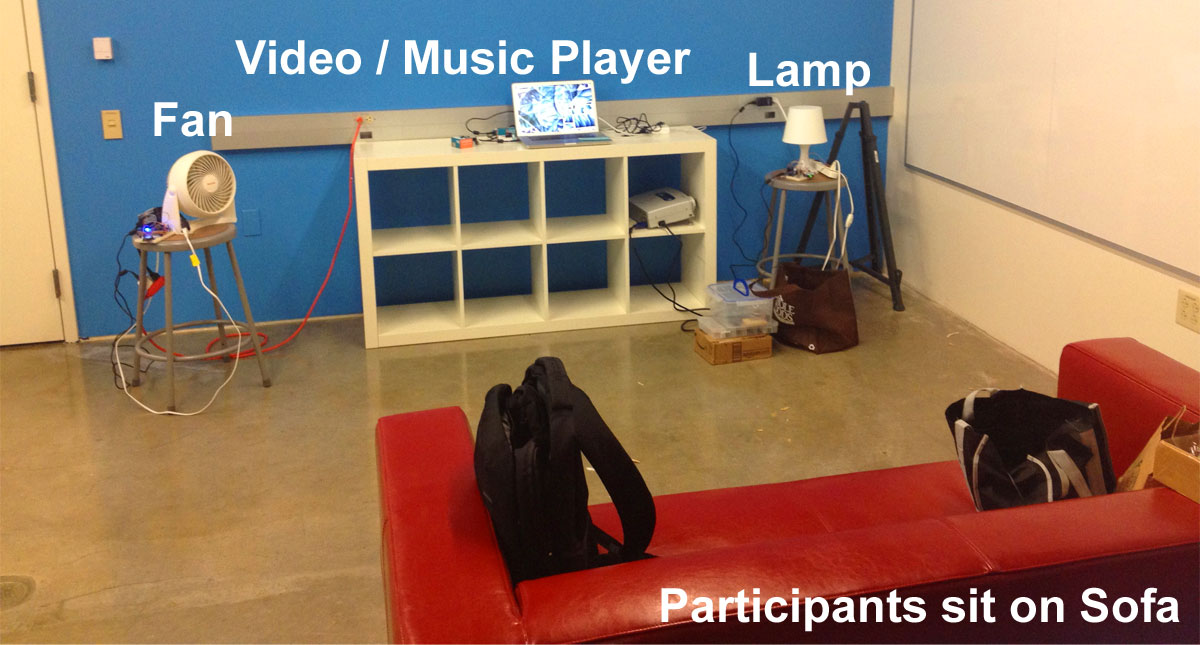
\includegraphics[width=1.0\columnwidth]{figures/smarthome-scenario.jpg}
\caption{In the smart home scenario, participants completed a series of appliance control tasks in a simulated living room.}
\label{fig:smarthome}
\end{figure}

\subsection{Methodology}
We recreated a living room environment that had three controllable appliances: a fan, a lamp, and one laptop functioning as a video player (see Figure~\ref{fig:smarthome}). The fan and lamp had binary controls: they could be switched on or off. The laptop had multiple parameterized functions: participants could start, pause, fast forward, rewind, and adjust volume.

We then asked users to work through the following script for controlling the room for watching a movie in the evening:
{\small
\begin{enumerate}
\item Turn off the lights as you want to watch the movie in a darkened room.
\item You feel a little hot in the room, so you turn on the fan.
\item You connect to the Smart TV and start playing the movie. 
\item The volume seems too soft to hear over the fan- turn it up a bit. 
\item After a while, you want to take a break to get a snack. Pause the movie. 
\item When you come back, you've forgotten what was said last - rewind by ~30 seconds and restart the movie. 
\item When the credits roll, you stop the movie and turn the lights back on.
\item After awhile, you turn off the fan and leave the room.
\end{enumerate}
}

For this study, we only elicited subjective data in the form of Likert data and open-ended responses.
\begin{figure}[t]
\centering
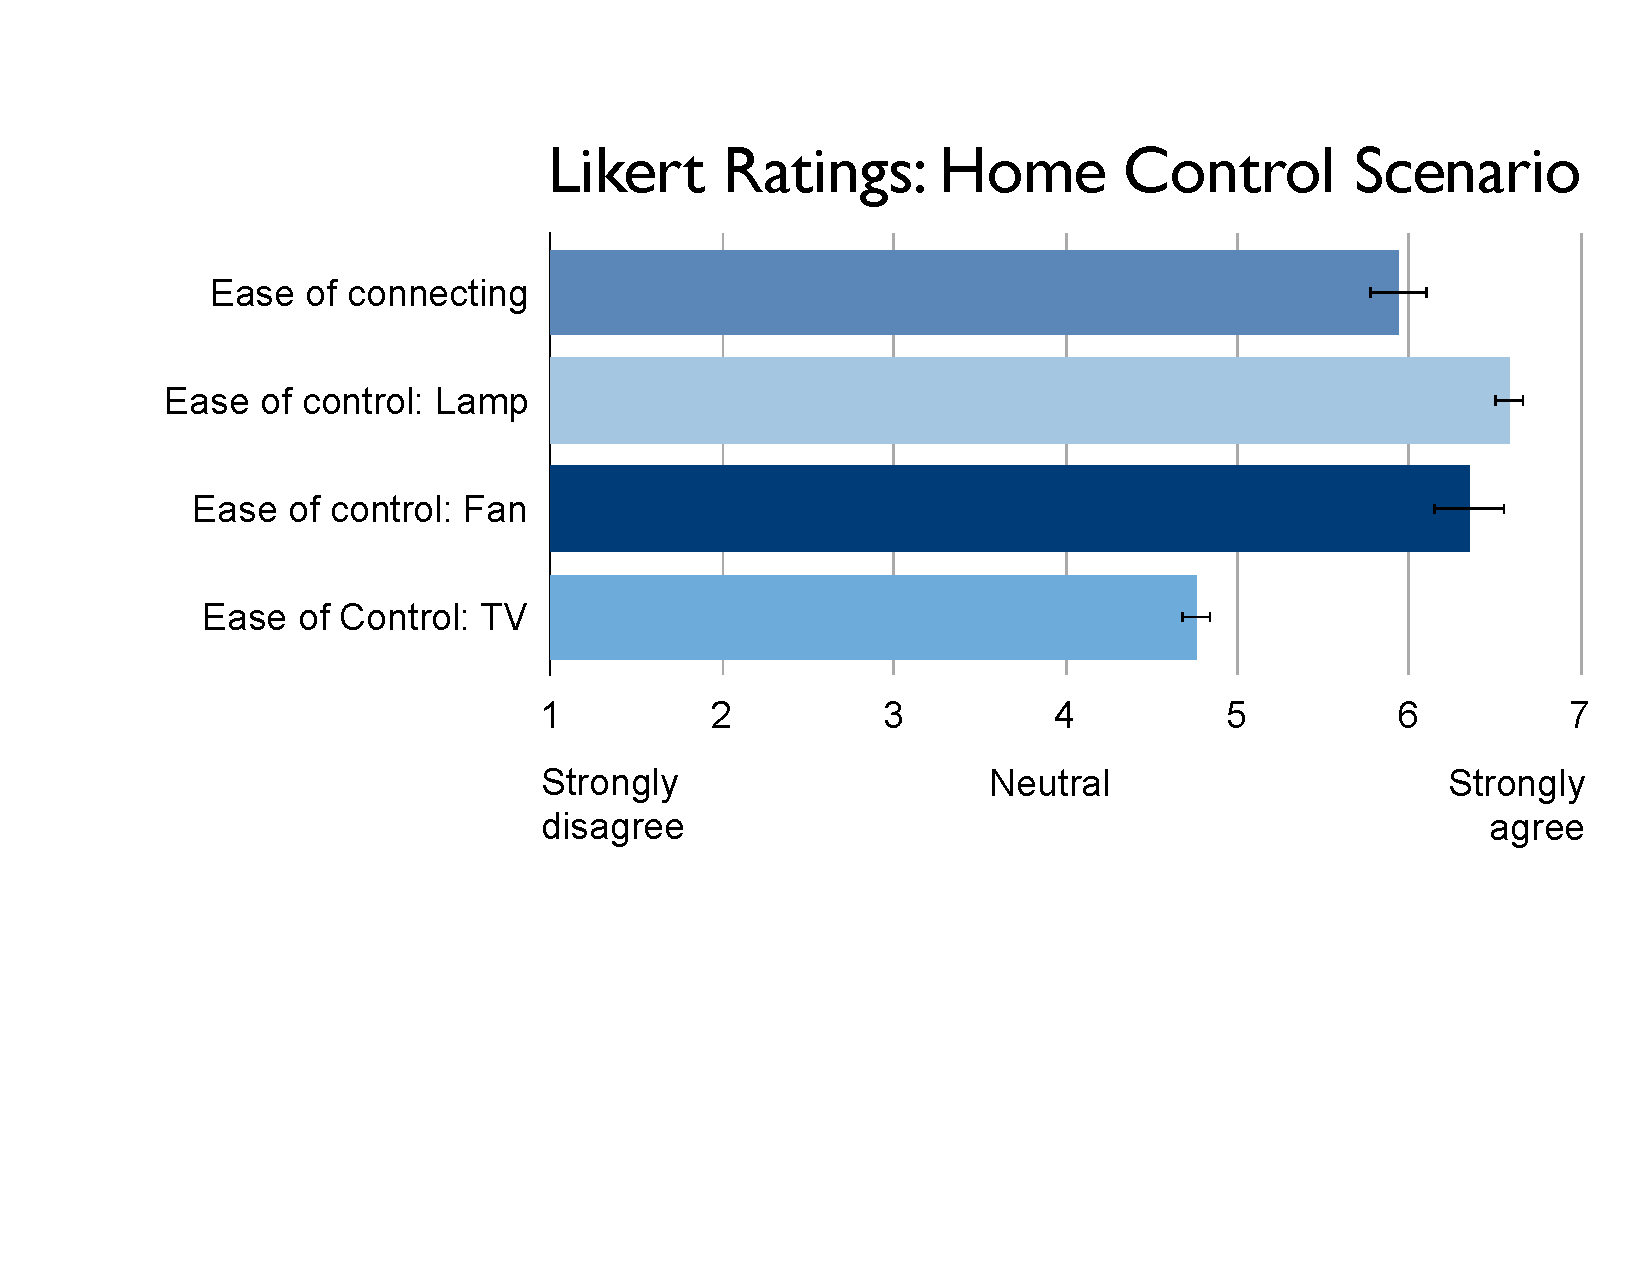
\includegraphics[width=1.0\columnwidth]{figures/scenario-likert.pdf}
\caption{Likert scale ratings for ease of use of aspects of the smart home control scenario. Error bars show standard error.}
\label{fig:smarthome-likert}
\end{figure}

\subsection{Results}
All participants successfully completed the list of tasks. They commented positively on the universal remote control functionality (e.g., \studyquote{I didn't have to search for different remote controllers for different appliances}) and stated it was easy to target and connect to appliances, in line with the findings of the previous study procedure. Participants saw benefits of the device for families --- \studyquote{ It might also be useful for people who need to take care of small children that they can complete all the tasks while keeping an eye on their children at the same time}, though settings that require more movement than watching a movie at home (e.g., cooking) may be more appropriate scenarios for wearing the device. 

\subsubsection{Simple and Complex Controls}
Participants rated the ease of control of particular appliances differently. Ease of use ratings were higher for the lamp and fan which had simple, discrete on/off actions, and lower for the more complex movie player (see Figure~\ref{fig:smarthome-likert}). Multiple participants remarked that the difficulty was based on the affordances of Glass: \studyquote{Most of the difficulty I had with Glass came from having to navigate the interface on the tiny screen with the touch pad}. The screen size and (largely) 1D input put a limit on the complexity of interfaces that can be presented. As one participant remarked: \studyquote{[The media player] does not seem to be more efficient than a tablet device.} The difficulty can also partly be ascribed to our interaction design, which required one finger swipes to switch between parameters and two finger gestures for adjusting parameters --- it was hard for users to exert fine control over two-finger swipes. In addition, users did not always remember these mappings as they are not yet part of a standard gesture vocabulary.

\subsubsection{Eliminating Steps}
Participants liked the efficiency of our design but also suggested further simplification by eliminating the explicit connection step, they wanted to immediately connect to any appliance that receives the infrared signal --- \studyquote{I intuitively want the screen to automatically appear when the IR detects the appliance rather than having to tap to connect.} Such a design would increase the efficiency of interaction, but at a power tradeoff, as the wireless radio will have to send and receive data each time the user looks at a device --- whether on purpose or inadvertently. We leave the study of battery life implications of interaction design choices to future work. 

\subsubsection{Feedback On Screen or In The World}
We found out that the near-eye display may occlude or overlap the target appliance when a participant looks at a target. This may make it difficult to read either the on-screen display or see information displayed on the target device.  As one participant remarked \studyquote{This was especially annoying with the TV because there were two screens overlapping each other.} While it is possible to look away once a device has been acquired to better see the Glass display, a tension remains whether users should rely on feedback from the appliances themselves or on the near-eye display.


 % discussion
\section{Discussion}
Our study procedures demonstrated that users can successfully select and control smart appliances with head-worn infrared targeting, and that this technique outperforms list selection on the Google Glass wearable device. In this section, we revisit some of the results and observations and discuss their larger significance and potential paths for future work.

\paragraph{Meaningful Results?}
While the performance increase in our targeting study is statistically significant, readers may wonder whether it is truly meaningful. We believe it is, for two reasons: first, our technique avoids the problems of {\em naming} and {\em scoping} inherent in any interface that uses representations of objects (e.g., a list of identifiers) rather than the objects themselves. We argue that this disintermediation of interaction leads to a cognitively simpler design. Second, our existing study only showed results for a modest number of targets. Our technique should have a wider margin as the number of targets increases. Of course, the number of targets one can realistically expect may vary across application domains.

\paragraph{Hands-Free Operation}
While head movement is not as precise as hand positioning (e.g., in Patel's mobile laser pointing~\cite{patel_2-way_2003}), one key benefit of our target acquisition step is that it does not require the user's hands. This raises the question if the rest of the interaction (disambiguation and device control) could also be achieved in a hands-free fashion. Voice-command control is an obvious candidate, though such approaches have not found widespread adoption because of social acceptability and other factors.

\paragraph{Hardware Limitations}
In our prototype, the IR emitter is fixed in a single position. Due to different sizes and shapes of the users’ heads, the emitter may not line up exactly with their head orientation. An adjustable emitter (paired with a suitable calibration routing) would improve the performance of our design. Some of our users also mentioned that they had to move closer to some targets to successfully select them. A stronger emitter could overcome these problems, but care has to be taken to avoid possible reflection problems where IR light bounces off a wall and hits an unintended target behind the user.

More importantly though, the main limitation of our design is that extra hardware for infrared communication is needed for the head-mounted device and each controllable appliance. One potential approach to sidestep this requirement would be to combine the growing availability of high-resolution indoor maps with live data from the point-of-view camera on the device to determine what a user is looking at without any infrared data exchange.

\paragraph{The Midas Look}
Our participants suggested eliminating explicit initiation of a connection by the user. However, one of the design guidelines for near-eye displays is to avoid pushing information to the display without an initial request from the user --- flashing device information on screen each time a user moves their head would surely be counterproductive. Future work should investigate how to intelligently decide when and how to initiate interaction for the user.

\paragraph{Where is the Target?}
One open design question of our approach is where infrared receivers should be placed. For a light, one might put a received on the light itself, or on the light switch, to cater to existing expectations. For volume control, the infrared receiver might be located on a speaker or on the amplifier. A thorough study of user preferences would be interesting; though we also point out that our architecture could easily support multiple receivers that end up controlling the same appliance.


 % conclusion
\section{Conclusion}
We introduced a novel method for selecting and controlling smart appliances in physical spaces through infrared targeting based on head orientation. Through our solution, we attempt to address the naming and scaling challenges faced by handheld mobile devices. The design takes advantage of the fact that visual attention can express intention. The visual feedback provided by the target appliances helps users keep their focus in the physical world. While we present a prototype approach that requires that the user carry additional hardware, all parts can readily be miniaturized and integrated into future head-worn hardware. We also introduced a disambiguation technique in case head orientation is not sufficient to determine a unique target. We characterized our devices performance, arguing that it is matched well to the amount of head movement people can control without strain. A target acquisition study showed that the technique is efficient; a home control scenario showed promise but also limitations when trying to control complex appliances. As our environment continues to be populated by a swarm of sensing and actuation devices, methods to interrogate and control our smart environments will become increasingly important.


\balance

\bibliographystyle{acm-sigchi}
\begin{thebibliography}{10}

\bibitem{azuma_recent_2001}
Azuma, R., Baillot, Y., Behringer, R., Feiner, S., Julier, S., and {MacIntyre},
  B.
\newblock Recent advances in augmented reality.
\newblock {\em {IEEE} Comput. Graph. Appl. 21}, 6 (Nov. 2001), 34–47.

\bibitem{beigl_point_1999}
Beigl, M.
\newblock Point \& click-interaction in smart environments.
\newblock In {\em Handheld and Ubiquitous Computing}, H.-W. Gellersen, Ed.,
  no.~1707 in Lecture Notes in Computer Science. Springer Berlin Heidelberg,
  Jan. 1999, 311--313.

\bibitem{card_morphological_1991}
Card, S.~K., Mackinlay, J.~D., and Robertson, G.~G.
\newblock A morphological analysis of the design space of input devices.
\newblock {\em {ACM} Trans. Inf. Syst. 9}, 2 (Apr. 1991), 99–122.

\bibitem{costanza_sensortune:_2010}
Costanza, E., Panchard, J., Zufferey, G., Nembrini, J., Freudiger, J., Huang,
  J., and Hubaux, J.-P.
\newblock {SensorTune:} a mobile auditory interface for {DIY} wireless sensor
  networks.
\newblock In {\em Proceedings of the {SIGCHI} Conference on Human Factors in
  Computing Systems}, {CHI} '10, {ACM} (New York, {NY}, {USA}, 2010),
  2317–2326.

\bibitem{cross_low-cost_2012}
Cross, A., Cutrell, E., and Thies, W.
\newblock Low-cost audience polling using computer vision.
\newblock In {\em Proceedings of the 25th annual {ACM} symposium on User
  interface software and technology}, {UIST} '12, {ACM} (New York, {NY}, {USA},
  2012), 45–54.

\bibitem{kemp_point-and-click_2008}
Kemp, C.~C., Anderson, C.~D., Nguyen, H., Trevor, A.~J., and Xu, Z.
\newblock A point-and-click interface for the real world: laser designation of
  objects for mobile manipulation.
\newblock In {\em Proceedings of the 3rd {ACM/IEEE} international conference on
  Human robot interaction}, {HRI} '08, {ACM} (New York, {NY}, {USA}, 2008),
  241–248.

\bibitem{lifton_tricorder:_2007}
Lifton, J., Mittal, M., Lapinski, M., and Paradiso, J.~A.
\newblock Tricorder: A mobile sensor network browser.
\newblock In {\em Proceedings of the {ACM} {CHI} 2007 Conference-Mobile Spatial
  Interaction Workshop} (2007).

\bibitem{mittal_ubicorder:_2011}
Mittal, M., and Paradiso, J.
\newblock Ubicorder: A mobile device for situated interactions with sensor
  networks.
\newblock {\em Sensors Journal, {IEEE} 11}, 3 (2011), 818--828.

\bibitem{myers_interacting_2002}
Myers, B.~A., Bhatnagar, R., Nichols, J., Peck, C.~H., Kong, D., Miller, R.,
  and Long, A.~C.
\newblock Interacting at a distance: measuring the performance of laser
  pointers and other devices.
\newblock In {\em Proceedings of the {SIGCHI} Conference on Human Factors in
  Computing Systems}, {CHI} '02, {ACM} (New York, {NY}, {USA}, 2002), 33–40.

\bibitem{pausch_user_1993}
Pausch, R., Shackelford, M.~A., and Proffitt, D.
\newblock A user study comparing head-mounted and stationary displays.
\newblock In {\em Virtual Reality, 1993. Proceedings., {IEEE} 1993 Symposium on
  Research Frontiers in} (1993), 41–45.

\bibitem{raskar_rfig_2004}
Raskar, R., Beardsley, P., van Baar, J., Wang, Y., Dietz, P., Lee, J., Leigh,
  D., and Willwacher, T.
\newblock {RFIG} lamps: interacting with a self-describing world via
  photosensing wireless tags and projectors.
\newblock In {\em {ACM} {SIGGRAPH} 2004 Papers}, {SIGGRAPH} '04, {ACM} (New
  York, {NY}, {USA}, 2004), 406–415.

\bibitem{rukzio_experimental_2006}
Rukzio, E., Leichtenstern, K., Callaghan, V., Holleis, P., Schmidt, A., and
  Chin, J.
\newblock An experimental comparison of physical mobile interaction techniques:
  Touching, pointing and scanning.
\newblock In {\em {UbiComp} 2006: Ubiquitous Computing}. Springer, 2006,
  87–104.

\bibitem{schmidt_picontrol:_2012}
Schmidt, D., Molyneaux, D., and Cao, X.
\newblock {PICOntrol:} using a handheld projector for direct control of
  physical devices through visible light.
\newblock In {\em Proceedings of the 25th annual {ACM} symposium on User
  interface software and technology}, {UIST} '12, {ACM} (New York, {NY}, {USA},
  2012), 379–388.

\bibitem{patel_2-way_2003}
Shwetak N.~Patel, G. D.~A.
\newblock A 2-way laser-assisted selection scheme for handhelds in a physical
  environment.
\newblock 200--207.

\bibitem{weiser_coming_1997}
Weiser, M., and Brown, J.~S.
\newblock The coming age of calm technolgy.
\newblock In {\em Beyond calculation}, P.~J. Denning and R.~M. Metcalfe, Eds.
  Copernicus, New York, {NY}, {USA}, 1997, 75–85.

\bibitem{willis_sidebyside:_2011}
Willis, K.~D., Poupyrev, I., Hudson, S.~E., and Mahler, M.
\newblock {SideBySide:} ad-hoc multi-user interaction with handheld projectors.
\newblock In {\em Proceedings of the 24th annual {ACM} symposium on User
  interface software and technology}, {UIST} '11, {ACM} (New York, {NY}, {USA},
  2011), 431–440.

\bibitem{wilson_xwand:_2003}
Wilson, A., and Shafer, S.
\newblock {XWand:} {UI} for intelligent spaces.
\newblock In {\em Proceedings of the {SIGCHI} Conference on Human Factors in
  Computing Systems}, {CHI} '03, {ACM} (New York, {NY}, {USA}, 2003),
  545–552.

\end{thebibliography}

\end{document}
